\documentclass[tikz,border=3pt]{standalone}
\usetikzlibrary{arrows.meta,positioning,shapes.geometric}

\begin{document}
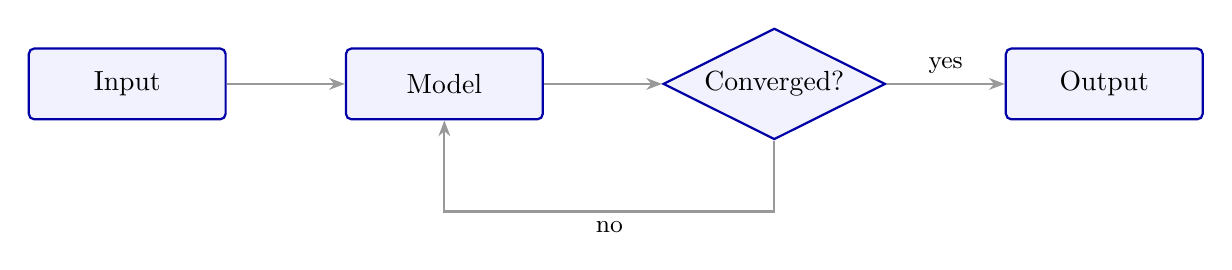
\begin{tikzpicture}[
  node distance=1.35cm and 1.5cm,
  block/.style={draw=blue!65!black, fill=blue!5, rounded corners=2pt, thick,
    minimum width=2.5cm, minimum height=9mm, align=center},
  decision/.style={diamond, draw=blue!65!black, fill=blue!5, thick,
    aspect=2, inner sep=2pt, align=center},
  flow/.style={-{Stealth[length=2mm]}, draw=gray!80, thick},
]
  \node[block] (input) {Input};
  \node[block, right=of input] (model) {Model};
  \node[decision, right=of model] (check) {Converged?};
  \node[block, right=of check] (output) {Output};
  \draw[flow] (input) -- (model);
  \draw[flow] (model) -- (check);
  \draw[flow] (check) -- node[above, font=\small] {yes} (output);
  \draw[flow] (check.south) -- ++(0,-0.9) -| node[pos=0.25, below, font=\small] {no} (model.south);
\end{tikzpicture}
\end{document}
